\cxset{style38/.style={
 name=,
 numbering=arabic,
 number font-size= huge,
 number font-family= rmfamily,
 number font-weight= normalfont,
 number before=,
 number position=rightname,
 number after =,
 number display=inline,
 number float=center,
 chapter font-family= sffamily,
 chapter font-weight= mdweight,
 chapter spaceout=none,
 number after={\vspace*{6.5pt}\par},
 chapter before=\par,
 chapter after=\par,
 chapter color= black!90,
 number color=black!90,
 title beforeskip={},
 title afterskip={\vspace{50pt}},
 title before=\par,
 title after=\par,
 title display=block,
 title font-family= rmfamily,
 title font-color= black!80,
 title font-weight=mdseries,
 title font-size= huge,
 chapter title align=centering,
 chapter title text-align=center,
 chapter title width=\textwidth,
 chapter font-size=,
}}

\cxset{style38,
       author block=true,
       author block format=\par\leavevmode\vskip20pt\centering\normalfont\itshape,
       author names=Yiannis Lazarides}
\chapter{STAGES OF INITIATION IN THE  ELEUSINIAN AND SAMOTHRACIAN MYSTERIES STYLE THIRTY EIGHT}

This style uses rules to enclose both the chapter name and number as well as the title, which necessarily needs to be rather short.
\medskip

\begin{figure}[ht]
\centering
\fbox{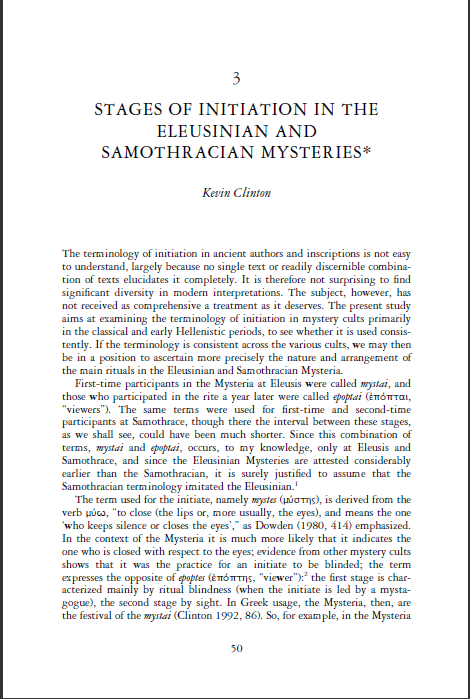
\includegraphics[width=0.6\textwidth]{./chapters/chapter38.png}}
\end{figure}

